
\begin{frame}[plain]
  \titlepage
\end{frame}

\begin{frame}{Содержание}
  \tableofcontents
  % You might wish to add the option [pausesections]
\end{frame}
\section{Активные молекулы}

\begin{frame}{Активные молекулы}{}
 \begin{itemize}
	\item В основном биологически активные молекулы взаимодействуют нековалентно с биополимерами
	\item Агонисты связываются как нативные лиганды и дают тот же эффект
	\item Антагонисты конкурируют или препятствуют связыванию нативного лиганда
	\item Обратные агонисты связываются и оказывают эффект, обратный эффекту нативного лиганда
	\item Хорошие молекулы показывают высокую комплементарность поверхности биополимера
 \end{itemize}
\end{frame}


\begin{frame}{Свойства лекарства}{}
 \begin{itemize}
\item     Лекарством обычно являются не только те молекулы, которые хорошо связываются с биополимером.
\item	  Лекарство должно иметь приемлемую растворимость
\item	  Часто бывает, что лекарству надо проникнуть сквозь мембрану.
\item	  Хорошо когда лекарство в итоге метаболизируется, а не накапливается в тканях.
	\end{itemize}
\end{frame}

\begin{frame}{Как искать активные молекулы?}
	\begin{itemize}
		\item	Можно пытаться искать вещества в биоматериалах. 
		\item	Можно проводить роботизированное сканирование библиотеки соединений на активность в разных тестах. 
		\item Недостаток сканирования: не все тесты можно адаптировать под робота.
		\item   Возможен высокий уровень шума из-за не специфических взаимодействий
		\item    Можно применить фильтрацию по подобию соединений, для этого нужны ИТ.
		\end{itemize}
	\end{frame}

\section{Фарминдустрия}
\begin{frame}{Особенности деятельности фарм-производителей}
    \textbf{Дженерик} - лекарство без патентной защиты (срок вышел)
    \vspace{1cm}
    \begin{itemize}
        \item Рынок высоко конкурентен.
        \item Разработка нового лекарства занимает от 10 до 20 лет.
        \item Новые лекарства приносят основную прибыль
        \item 4 основные фазы: открытие, разработка, испытания, продажи
    \end{itemize}
\end{frame}

\begin{frame}{R{\&}D}
\setchemfig{arrow coeff=0.7, arrow style={blue, thick}}
\setchemfig{compound style={draw,line width=0.8pt, semitransparent,
            text opacity=1,inner sep=5pt,rounded corners=1mm}}
%\setarrowdefault{,0.7,blue,thick} 
%\setcompoundstyle{draw,line width=0.8pt,semitransparent,text opacity=1,inner sep=5pt,rounded corners=1mm}
\schemestart
{Болезнь}\arrow([fill=red]--[fill=blue])[0]
{Белок}\arrow(--[fill=gray])[0]
{Ингибитор}\arrow(--[fill=green])[-160]
{Испытания на животных}\arrow(--[fill=yellow])[-90]
{Лекарство и масштабирование}\arrow(--[fill=magenta])[-160]
{Клинические испытания}\arrow(--[fill=cyan])[0]
{Подтверждение регулятором}%\arrow(--[draw=none])[-90]
\schemestop
\end{frame}

\begin{frame}{Новые технологии}
    \begin{itemize}
        \item Чипы: экспрессия генов.
        \item Структуры: роботизированный поиск комплексов с кристаллом белка.
        \item Высоко-производительный поиск ингибиторов.
        \item Виртуальный поиск.
        \item Комбинаторная химия.
    \end{itemize}
    \vspace{1cm}
    \textbf{Все это в основном относится к стадии поиска ингибитора}
\end{frame}

\begin{frame}{Как хемоинформатика может помочь?}
    \begin{itemize}
        \item Разработка методов и управление информацией о лигандах.
        \item Оценка данных \textit{in silico} для минимизации рисков.
            \begin{itemize}
                \item Разработка библиотеки.
                \item Виртуальный поиск.
                \item Оценка стоимости и выгоды.
            \end{itemize}
        \item Организация доступа к информации.
        \item Интеграция процессов.
    \end{itemize}
\end{frame}

\section{HTS}
\begin{frame}{Пример: HTS, Высоко-производительный поиск ингибиторов}
	\begin{center}
%    \setlength{\fboxsep}{1pt}
%    \fcolorbox{black}{white}
\\
    до 100000 соединений в день
	\end{center}

\end{frame}

\begin{frame}{HTS и поток данных}
    \begin{itemize}
        \item Исполнить HTS.
        \item Решить какие соединения активны а какие нет.    
        \item Кластеризация активных  соединений в классы.
        \item Визуализация.
        \item Идентификация "основы" для каждого класса.
        \item Поиск причин, элементов структуры, которые приводят к "не активности".
        \item Использование структурной информации для объяснения активности.
    \end{itemize}
\end{frame}


\begin{frame}{Пример, комбинаторная химия}
  \begin{itemize}
      \item Исследователи используют "строительные блоки" для быстрого создания большого количества разных  соединений.
    \vspace{1cm}
      \item Обычно используется некоторая "основа"  и "строительные блоки" присоединяются к разным местам основы.
   \end{itemize}
\end{frame}

\begin{frame}{Комбинаторная химия}
          "Основа" \hspace{3cm}"Блоки" \hspace{3cm} Примеры\\
    \begin{columns}[c]
        \begin{column}{.3\textwidth}
            \vspace{1cm}
 %           \setatomsep{2.0em}\setcrambond{2pt}{}{}%
            \chemfig[atom sep=2em]{*6(=(-R_1)-*5(--(-R_3)-N-)=-(-R_2)=-)}
        \end{column}
        \begin{column}{.4\textwidth}
            \small 
            R$_1$ = OH, OCH$_3$, NH$_2$, Cl, COOH \\
            \vspace{0.5cm}
            R$_2$ = Phe, OH, NH$_2$, Br, F,  CN \\
            \vspace{0.5cm}
            R$_3$ = CF$_3$, NO$_2$,  OCH$_3$,  OH , PheO 
        \end{column}
        \begin{column}{.3\textwidth}
   %         \setatomsep{2.0em}\setcrambond{2pt}{}{}%
            \tiny
            \chemfig[atom sep=2em]{*6(=(-O)-*5(--(-O-)-N-)=-(-Br)=-)}\\ 
            \vspace{0.2cm}
			\chemfig[atom sep=2em]{*6(=(-COO\ominus)-*5(--(-N(=[1]O)-[7]\chemabove{O}{\scriptstyle\hspace{2mm}\ominus})-N-)=-(-C~N)=-)} \\
            \vspace{0.2cm}
            \chemfig[atom sep=2em]{*6(=(-NH_2)-*5(--(-C(-[2]F)(-[6]F)-F)-N-)=-(-F)=-)} \\
        \end{column}
    \end{columns}
\end{frame}   

\begin{frame}{Хемоинформатика и библиотеки}
    \begin{itemize}
        \item Какие блоки выбрать?
        \item Какие библиотеки строить?
            \begin{itemize}
                \item Дополнение известных  наборов
                \item Модификация под конкретный белок
                \item Полное "насыщение" библиотеки
            \end{itemize}
        \item Компьютерное профилирование библиотеки
            \begin{itemize}
                \item Виртуальными библиотеками удобно манипулировать на компьютере
            \end{itemize}
    \end{itemize}
\end{frame}



\section{Хемоинформатика}

\begin{frame}[fragile]{Компьютерное представление молекул}
	\begin{itemize}
		\item Хранение в компьютере молекулы как изображения имеет малую ценность
		\item Большинство современных баз данных представляет молекулу как граф, с узлами и рёбрами
		\item Графы представляются как таблицы связей. 
	\end{itemize}
	\small
\begin{verbatim}
Marvin  04200617372D          
  4  3  0  0  0  0            999 V2000 
    0.0000    0.0000    0.0000 C   0  0  0  0  0  0  0  0  0  0  0  0
    0.7145   -0.4125    0.0000 O   0  0  0  0  0  0  0  0  0  0  0  0
   -0.7145   -0.4125    0.0000 C   0  0  0  0  0  0  0  0  0  0  0  0
    0.0000    0.8250    0.0000 O   0  0  0  0  0  0  0  0  0  0  0  0
  1  4  2  0  0  0  0
  2  1  1  0  0  0  0
  3  1  1  0  0  0  0
M  END  
\end{verbatim}

\end{frame}

\begin{frame}[fragile]{Линейное представление молекул, SMILES}
Молекула представляется в виде диаграммы и \\
каждый атом проходится только один раз 
\footnotesize
\begin{center}
\begin{tabular}{c c c c}%
		 \hline
		 CC & ethane & {[OH3+]} & hydronium ion \\
			 O=C=O & carbon dioxide & [[2H]]O[[2H]] & deuterium oxide \\
		 C{\#}N & hydrogen cyanide & [[235U]] & uranium-235 \\
CCN(CC)CC & triethylamine & F/C=C/F & E-difluoroethene \\
	 CC(=O)O & acetic acid & F/C=C\slash F & Z-difluoroethene \\
 C1CCCCC1 & cyclohexane & N[[C@@H]](C)C(=O)O & L-alanine \\
		c1ccccc1 & benzene & N[[C@H]](C)C(=O)O & D-alanine \\
	 \hline
\end{tabular}
\end{center}
	 \vspace{0.5cm}
\normalsize
\begin{center}
    \textbf{Реакции в виде SMILES}
\small

\begin{tabular}{c c}%
\hline
{[I-].[Na+]}.C=CCBr >> {[Na+].[Br-]}.C=CCI &  реакция замещения\\
{(C(=O)O).(OCC)>>(C(=O)OCC).(O)}    &     образование сложного эфира\\
\end{tabular}
\end{center}
\end{frame}


\begin{frame}{Стандартизация SMILES}
	\begin{itemize}
		\item  Очевидно, что одну молекулу можно описать разными способами.
		\item Морган в 1965 году предложил рассматривать каждый атом по свойству его окружения. 
		\item  Стандартные SMILES называют Unique.
	\end{itemize}
	\begin{center}
		\begin{tabular}{c c}
	\hline
	Input SMILES	&	Unique SMILES \\
	\hline
		OCC			&	CCO \\
     {[CH3][CH2][OH]}	&	CCO\\
	   C-C-O			&	CCO\\
	C(O)C			&	CCO\\
OC(=O)C(Br)(Cl)N &	NC(Cl)(Br)C(=O)O\\
ClC(Br)(N)C(=O)O &	NC(Cl)(Br)C(=O)O\\
O=C(O)C(N)(Br)Cl &	NC(Cl)(Br)C(=O)O\\
	\hline
\end{tabular}
	\end{center}
\end{frame}

\begin{frame}{Описание SMILES: атомы}
	\begin{itemize}
		\item	 Одно буквенные атомы, а именно :  B, C, N, O, P, S, F, Cl, Br,  I записываются как есть, как один символ.
		\item  Все остальные атомы записываются в квадратных скобках [Pt]
		\item  Так как атомы водорода обычно не указываются, то “валентность” атомов определятся как наименьшая из ближайших Т.е.  B (3), C (4), N (3,5), O (2), P (3,5), S (2,4,6).
		\item   “Валентности”, отличные от “нормальных”, указывают в скобках [S], [H+], [Fe+2], [OH-], [Fe++], [OH3+], [NH4+]
		\end{itemize}
\end{frame}


\begin{frame}[fragile]{Описание SMILES: связи}
\begin{center}
	\begin{tabular}{c c}
		\hline
	CC & этан \\
	C=C & этилен\\
	O=C=O &  CO2 \\
	C{\#}N & HCN \\
	CCO & этанол \\
	{[H][H]}  & водород \\
		\hline
	\end{tabular}
\end{center}
	\vspace{1cm}
	Ветвление цепи отображается в скобках () \\
	Пример: ССС(СС)СОО
\end{frame}

\begin{frame}{Описание SMILES: циклы}
	\begin{itemize}
		\item C1CCCCC1 циклогексан
	\vspace{0.1cm}
\setchemfig{arrow coeff=0.7,arrow style={black, thick}}
\schemestart
\chemfig[atom sep=2em]{C-*6(=-(-Br)----)} \arrow
%\setatomsep{2.0em}\setcrambond{2pt}{}{}%
\chemfig[atom sep=2em]{@{c}C-**[-180,90,dash pattern=on 1pt off 1pt, ->,thick, blue!50!white]6(@{a}=-(-@{d}Br)---@{b})}       
  \chemmove{%
%     \draw[->,thick, dash pattern= on 1pt off 1pt,blue,shorten >=6pt,shorten <=10pt](a).. controls +(-45:15mm) and
%     +(-20:15mm).. node[left]{$\boldsymbol{(a)}$}(b);
     \draw[->,red!50!white,thick, dash pattern= on 1pt off 1pt,shorten >=6pt,shorten <=10pt](c).. controls +(-15:15mm) and
     +(180:15mm).. node[left]{}(d);
     %\setchemrel{}{}{20pt}
}
\arrow(bb--foo[fill=blue!50!white,semitransparent,text opacity=1,inner sep=2mm,rounded corners=2mm])[15]\small{a) CC1=CC(Br)CCC1} 
\arrow(@bb--f[fill=red!50!white,semitransparent,text opacity=1,inner sep=2mm,rounded corners=2mm])[-15]\small{b) CC1=CC(CCC1)Br} 
\schemestop
\vspace{.1cm}
		\item	 Или более сложный пример:
\schemestart
\chemfig[atom sep=2em]{A?[1](-[7]E?[3]-F?[5]-[6]G?[4]-[4]H?[2]?[3])-B?[5]-[6]C?[4]-[4]D?[1]?[2]}
\arrow
\chemfig[atom sep=2em]{A?[1](-[7]E?[3]-[,,,,red,thick]F?[5]-[6,,,,red,thick]G?[4]-[4,,,,red,thick]H?[2]?[3])-[,,,,red,thick]B?[5]-[6,,,,red,thick]C?[4]-[4,,,,red,thick]D?[1]?[2,1,thick,red]}
    \arrow(--foo[fill=green,semitransparent,text opacity=1,inner sep=2mm,rounded corners=2mm])\small{A14B2C3D1H5G3F2E45} 
\schemestop

	\end{itemize}
\end{frame}


\begin{frame}{Описание SMILES: ароматика}
	\begin{itemize}
		\item SMILES для определения ароматичности использует расширенный алгоритм Хюккеля.
			\item  с1ссссс1 eq С1=СС=СС=C1 тут все атомы находятся в sp2-гибридизации
			\item с1сссс1 eq C1=CC=CC1 , последний атом в гибридизации sp3.
			\item			     Ароматичными могут быть атомы: C, N, O, P, S, As, Se, и *.
			\item				 Пример: c1cnc[nH]c(=O)1
\end{itemize}

\begin{center}
 	\chemfig{[:-30]N**6(--N-(=O)---)}	\hspace{.5cm} \normalsize
\end{center}
\end{frame}

\begin{frame}[fragile]{Структуры где есть нековалентные связи}
	\begin{center}
	\chemfig{[:-30]**6(---(-O{^\ominus} \quad Na{^\oplus} )---)}\\
	\vspace{1cm}
В SMILES нотации это:\\
{[Na+]}.{[O-]}c1ccccc1  \\
или \\
c1cc({[O-].[Na+]})ccc1
\end{center}
\end{frame}

\begin{frame}[fragile]{Изомеры}
  \begin{tabular}{c c c}
	  Изотопы &  ---  &  
  \begin{minipage}{4cm}\small
[12C],[13C]
  \end{minipage}   	  \\
  Цис-Транс & \tiny{\chemfig{F-[1]C=C-[1]F}} & 
	  \begin{minipage}{4cm}\small
          F/C=F/C или  F$\backslash$C=F$\backslash$C 
\end{minipage}  \\
	  Хиральность  & \tiny{\chemfig{H_3C>:([2]<NH_2)([6]-H)([0]-COOH)}
      \quad\chemfig{H_3C-o([7]-H)([1]-COOH)} } & 
	  \begin{minipage}{4cm}\small
N[C@](C)(C(=O)0)H \\
N[C@@](C)(H)C(=O)O
	  \end{minipage}  \\
	\end{tabular}
\end{frame}
   


\begin{frame}{SMARTS: паттерны для SMILES}
	 В принципе, SMARTS это SMILES + операторы логики и варианты в позициях.\\
	 \textbf{Пример для атомов: }\\
	 \begin{center}
	 \begin{tabular}{c c}
		 \hline
		 C & алифатический углерод \\
	  c & ароматический углерод \\
	  a & любой ароматический атом \\
   {[\#6]} & любой атом углерода\\
	{[++]} & атом с зарядом +2\\
	{[R]} & атом в кольце\\
   {[D3]} & атом с тремя связями ( не с атомами водорода)\\
   {[X3]} & атом с тремя связями, включая атомы водорода\\
   {[v3]} & атом с валентностью 3.\\
		 \hline
	 \end{tabular}
	 \end{center}
\end{frame}


\begin{frame}{SMARTS: логические операторы и примеры}
    \begin{center}
	\textbf{Логика:} \\
	\vspace{0.5cm}
	\begin{tabular}{c c}
	\hline
	!e1		& not e1\\
	e1{\&} e2	& a1 and e2\\ 
	e1,e2	& e1 or e2\\
	e1;e2	& a1 and e2 \\
		\hline
	\end{tabular}
	\vspace{0.5cm} \\
	\textbf{Пример:} \\
	\vspace{0.5cm}
	\begin{tabular}{c c}
		\hline
{[!C;R]} & не алифатический С в кольце\\
{[n;H1], [n\&H1], [nH1]} & Н в пирроле\\
{[c,n\&H1]} & С или Н в пирроле\\
{[X3\&H0]} & Атом с тремя связями не с Н\\
{[c,n;H1]} & N или С в связи с одним Н1\\
		\hline
	\end{tabular}
\end{center}
\end{frame}

\begin{frame}[fragile]{Линейное представление молекул,InChI  }
  InChI = IUPAC International Chemical Identifier \\
  Структура молекул описывается слоями :
  \begin{itemize}
      \item Основной слой содержит описание брутто формулы, связанности (c) и связей с водородами (h)\newline
          C2H6O/c1-2-3/h3H,2H2,1H3
      \item Слой с описанием заряда (p) кратности связей      
      \item Слой с описанием стереохимии и связей \newline
          C6H8O6/c7-1-2(8)5-3(9)4(10)6(11)12-5/h2,5,7-10H,1H2/t2-,5+
\end{itemize}
\centering \includegraphics[width=0.3\textwidth]{InChI}

\end{frame}

\section{QSAR}

\begin{frame}{Дискрипторы, правило Лепински}
    \begin{itemize}
        \item Водородные связи
        \item Гибкость молекулы
        \item Гидрофобность
     \end{itemize}        
     \vspace{0.5cm}
     {\Large Правило пяти Лепински}
    \begin{itemize}
        \item No more than 5 hydrogen bond donors 
        \item No more than 10 hydrogen bond acceptors 
        \item A molecular mass less than 500 daltons
        \item An octanol-water partition coefficient log P not greater than 5
     \end{itemize}        
\end{frame}

\begin{frame}{Поиск по 3D-базам данным}
	\begin{itemize}
		\item			 Поиск в 2D-пространстве хорош для поиска подобных  молекул, но биологически активные молекулы действуют благодаря специфической 3D-структуре.
		\item			Взаимодействие с биополимером может происходить благодаря нужному расположению в пространстве некоторых  групп. При этом различие в 2D-структуре может быть весьма существенным.
		\item			   Фармакофор — это набор свойств, которые являются общими для некоторой группы активных молекул.
		\item			    Пример:  Антигистаминный   3D-фармакофор 
	\end{itemize}

	\begin{center}
        \tiny
        \begin{tikzpicture}
            \node (n1)                {\chemfig{*6(=-=-=-)}};
             \node[below of = n1,yshift=-0.5cm] (n2) %{h};
             {\chemfig{*6(=\chembelow{}{[NC]}-=-=-)}};
             \node[below of = n1,yshift=0.15cm,xshift=2cm] (n3)
             {\chemfig{N([:60]-)([:-60]-)-}};
            \node[left of = n1,xshift=-3cm,text width=5cm] (n4) {{\normalsize Антигистаминный   3D-фармакофор }};
            \path[draw,dashed] (n1.center) -- (n2.center);
            \path[draw,dashed] (n1.center) -- (n3.west);
            \path[draw,dashed] (n2.center) -- (n3.west);
        \end{tikzpicture}
	\end{center}
\end{frame}

\begin{frame}[plain]
	\includegraphicsfs{pharmaco}
\end{frame}

\begin{frame}{Проблемы с фармакофорами}
	\begin{itemize}

\item Если молекулы более или менее подвижны, то это накладывает дополнительные требования на учёт конформационных превращений.
\item	 Для определения фармакофора надо определить, какой набор групп располагается в биополимере идентично.
\item	  Надо быть уверенным, что выбранный набор молекул  связывается с белком в одном и том же месте. Однозначное указание на это можно получить только экспериментально.
	\end{itemize}
\end{frame}

\begin{frame}{Систематический поиск}
	\begin{itemize}
		\item  Есть проблема: \newline
		%	  \setlength{\fboxsep}{10pt}
			   % \fcolorbox{}{}
		\item	Выбирают точки, которые по мнению исследователей определяют активность. Делают конформационный поиск для всех молекул. Если находят пересечения по геометрии, то на основе этих точек и геометрии пересечения формулируют фармакофор.
			\end{itemize}
		\end{frame}

\begin{frame}{Базы данных:}{}
 \begin{itemize}
  \item
  PubChem
\vspace{0.2cm}
  \item
  Cambridge database
\vspace{0.2cm}
  \item
   Inorganic structural database  
   \vspace{0.2cm}
 \end{itemize}
			  \setlength{\fboxsep}{0pt}
			    \fcolorbox{black}{white}{%
					\includegraphics[height=0.43\textheight]{pubchem1.png}
					\includegraphics[height=0.43\textheight]{pubchem2.png}
				}



\end{frame}
	
\begin{frame}[plain]
    %[fragile]{SOAP доступ к PubChem}
    \includegraphicsfs{pypubchem.png}
%  \begin{center}
  %  \tiny{
%\lstset{numbers=left, numberstyle=\tiny, stepnumber=1, numbersep=5pt}        
%	\includegraphics[width=1\textwidth]{pypubchem.png}

%}
%\end{center}
\end{frame}

\section{ML в  хемоинформатике}
\begin{frame}{ML в  хемоинформатике}
    \begin{itemize}
            \item Улучшение анализа HTS данных, в основном регрессии
            \item Улучшение предсказания  афиности, токсичности, фармокинетике для заданных соединений. Регресии и не только.
            \item Генерация новых  соединений под указанную задачу
        \end{itemize}
\end{frame}

\begin{frame}{Дескрипторы}
    \begin{itemize}
        \item 0D Формула: молекулярный вес, количество атомов и связей
        \item 1D Химические графы: фрагменты, функциональные группы 
        \item 2D Топология структуры: индексы  Weiner, Balaban, Randic, BCUTS
        \item 3D Геометрия молекулы:  WHIM, autocorrelation, 3D-MORSE, GETAWAY
        \item 4D Химическая информация:  Volsurf, GRID, Raptor
        \end{itemize}
\end{frame}


\begin{frame}{1D}
    \begin{itemize}
        \item Одномерные дескрипторы - это скаляры:  количество атомов, количество связей, молекулярный вес, суммы атомных свойств или количество фрагментов
        \item Просты в вычислении, страдают от проблем вырожденности, когда различные соединения сопоставляются с идентичными значениями дескриптора
        \item Одномерные дескрипторы обычно используются вместе с многомерными дескрипторами или выражаются как вектор из нескольких одномерных дескрипторов. 
     \end{itemize}
\end{frame}

\begin{frame}{2D}
    \begin{itemize}
        \item Двумерные химические дескрипторы являются наиболее частым типом дескрипторов
        \item Включают топологические индексы, молекулярные профили и двухмерные дескрипторы автокорреляции 
        \item Важной особенностью 2D-дескрипторов  является инвариантность графа, когда на значения дескрипторов не влияет перенумерация узлов (вершин) графа. 
        \item Cистема $Mold^2$ быстро генерирует до 200 типов 2D-дескрипторов для больших составных наборов данных. 
        \item Коммерческие программные пакеты  включают систему DRAGON, до 5000 декскрипторов. 
    \end{itemize}
\end{frame}

\begin{frame}{3D}
    \begin{itemize}
        \item 3D дескрипторы извлекают химические особенности из трехмерных геометрий  и наиболее чувствительны структурным изменениям 
        \item Могут  включать дескрипторы автокорреляции, данные об  заместителях , дескрипторы поверхности, объема и квантово-химические дескрипторы
        \item Трехмерные химические дескрипторы полезны для идентификации «каркасов» - отдельных химических каркасов со сходной связывающей активностью
        \item Ключевым ограничением является вычислительная сложность генерации конформеров и выравнивания структур
     \end{itemize}
\end{frame}
\begin{frame}{3D}
    \begin{itemize}
        \item Предсказанные конформации могут не соответствовать соответствующим биоактивным конформациям.
        \item Химические дескрипторы 4D являются расширением  дескрипторов 3D, которые одновременно рассматривают несколько структурных конформаций 
        \item  Эш и Фурчес применили MD киназы ERK2 для вычисления трехмерных дескрипторов по сеткой на основе траектории 20 нс и показали, что такие четырехмерные химические дескрипторы могут эффективно отличать наиболее активные ингибиторы ERK2 от неактивных с более высокой степенью обогащения. 
     \end{itemize}
\end{frame}

\begin{frame}{Fingerprints}
    \begin{itemize}
        \item FP это многомерные векторы, элементами которых являются значения химических дескрипторов 
        \item MACCS представляют собой двумерные двоичные FP (0 и 1), каждый из которых 166 бит указывает на наличие или отсутствие определенных ключей подструктуры
        \item Daylight FP и ECFP  позволяют извлекать патерны до определенной длины или диаметра из графа структуры, и  могут динамически
            индексировать представления с использованием хэш-функций, что  часто обеспечивают более высокую специфичность.
        \end{itemize}
\end{frame}


\begin{frame}{ECFP}
    \begin{center}
        \includegraphics[height=0.8\textheight]{ecfp-tr}\\

        \footnotesize 10.1021/ci100050t
    \end{center}
\end{frame}

\begin{frame}{Fingerprints}
    \begin{itemize}
        \item  Последние разработки - это continuous kernel  и встроенные нейронные FP. Это внутренние представления, полученные с помощью SVM и нейронных сетей.
        \item Duvenaud et al. распространил концепцию свертки на молекулы, представленные в виде двумерных молекулярных графов. 
        \end{itemize}
\end{frame}

\begin{frame}{3D fingerprints}
    \begin{itemize}
        \item 3D FP  включают химические характеристики, основанные на фармакофорных паттернах, свойствах поверхности, молекулярных объемах или взаимодействия молекул 
        \item MIF, реализованное в GRID. FP на основе MIF помещает лиганд в сетку с фиксированным интервалом и вычисляет электронный, стерический и гидрофобный вклад независимо в каждой точке сетки.
    \end{itemize}
\end{frame}

\begin{frame}{3D fingerprints}
    \begin{itemize}
        \item FP на основе MIF можно затем использовать в сравнительном анализе молекулярного поля (CoMFA) путем установления взаимосвязей между точками трехмерной сетки и активностями соединения. 
        \item Зависимость от относительной ориентации молекул внутри  сетки является основным ограничением.
        \item   Баскин и Жохова недавно представили подход непрерывного молекулярного поля (CMF), который заменяет сетку непрерывной функцией
    \end{itemize}
\end{frame}


\begin{frame}{SPLIF}
    \begin{center}
        \includegraphics[height=0.8\textheight]{splif-1.png}

        \footnotesize 10.1021/ci500319f
    \end{center}
\end{frame}
\begin{frame}{SPLIF}
    \begin{center}
        \includegraphics[height=0.8\textheight]{splif-2.png}
    \end{center}
\end{frame}


\begin{frame}{Ингибиторы киназ}
    \begin{itemize}
        \item Киназы ключевой класс ферментов в передаче сигналов
        \item Известно много ингибиторов киназ 
        \item Сайт связывания очень похож, это связывание ATP
     \end{itemize}
    \end{frame}

\begin{frame}{Interaction fingerprints}
    \begin{center}
    \includegraphics[height=.5\textheight]{chem-ifp} 
    \end{center}
    Включение мишень-специфичной  информации через IPF улучшило предсказание  связывания примерно на 10\% по сравнению с использованием
    традиционных FP. \\
    \footnotesize doi.org/10.1186/s13321-020-00434-7
\end{frame}

\begin{frame}{Features}
    \centering
    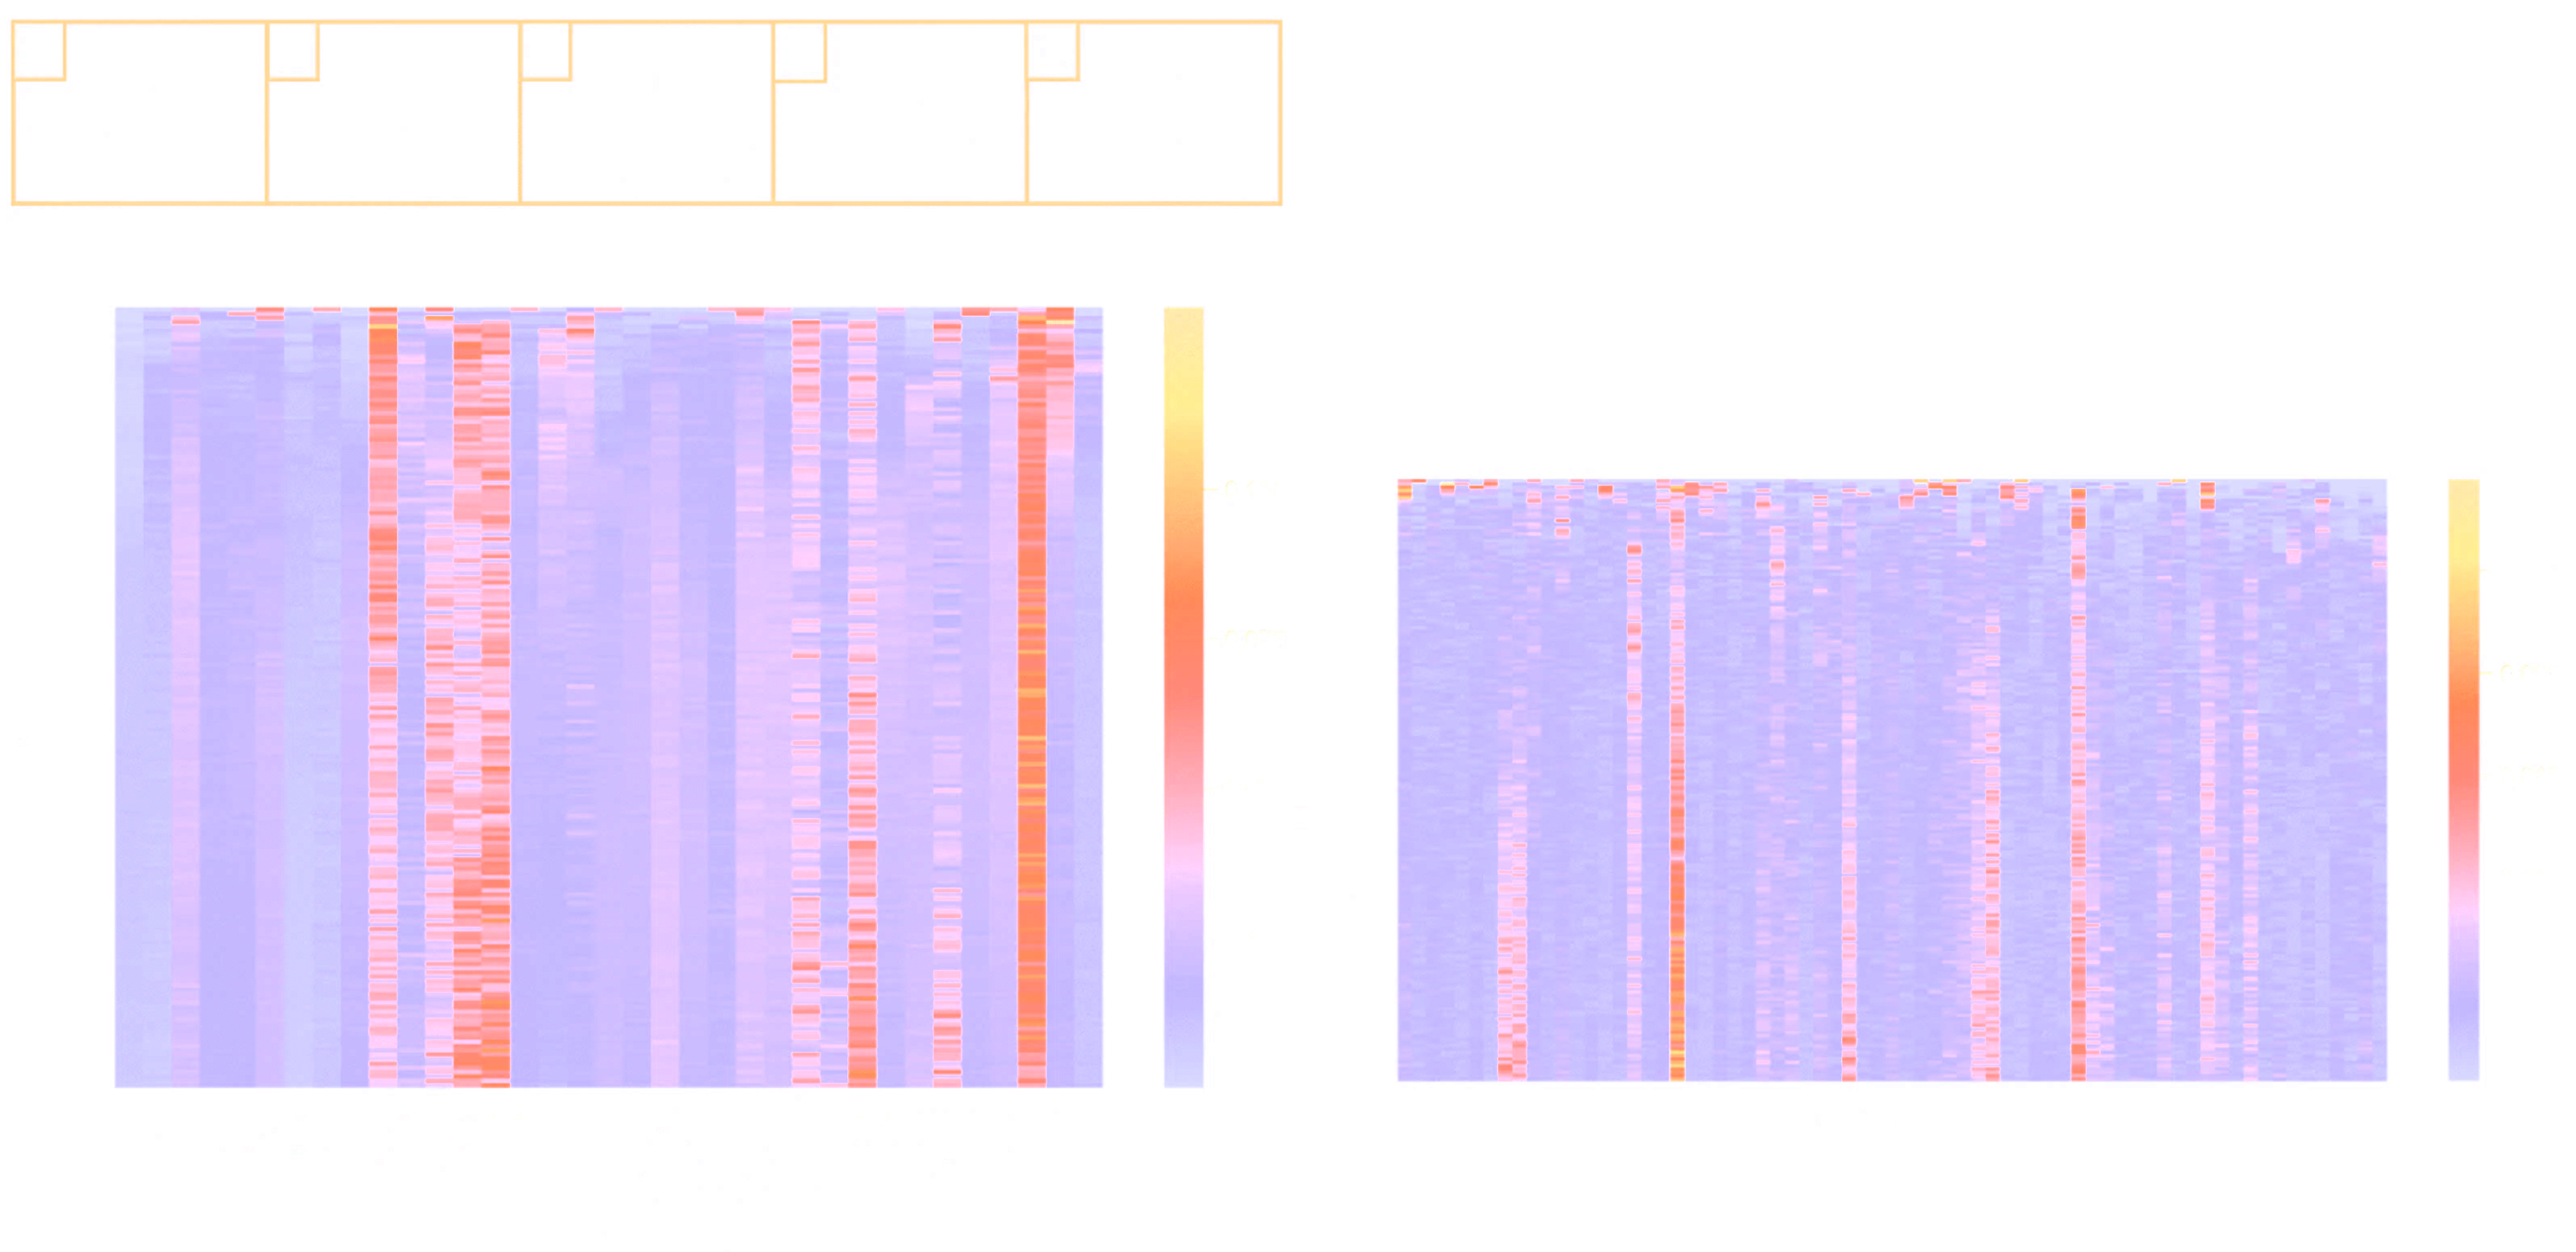
\includegraphics[height=.7\textheight]{chem-ifp-feat.png}\\
    \footnotesize doi.org/10.1186/s13321-020-00434-7
\end{frame}


\begin{frame}{Включение bioassay}
    \includegraphics[height=.6\textheight]{chem-assay.png}
    Комбинация структурных и данных об активности позволяет улучшить производительность и показывает эффективный переход между scafolds \\
    \footnotesize 10.1186/s13321-019-0376-1
\end{frame}

\section{Генеративные подходы}


\begin{frame}{Агент}
    \includegraphics[width=.99\textwidth]{chem-gen-agent.png}
    doi.org/10.1186/s13321-017-0235-x
\end{frame}
\begin{frame}{Генерация по подобию}
    \includegraphics[width=.99\textwidth]{chem-gen-agent2.png}
    doi.org/10.1186/s13321-017-0235-x
\end{frame}

\begin{frame}{ Generative Autoencoder}
    \includegraphics[height=.8\textheight]{chem-gen-ae}\\
    разработан для использования с RNN
\end{frame}

\begin{frame}{AE и GAN}
    \begin{itemize}
        \item Предварительно обученный автокодер использовался для сопоставления молекулярной структуры с латентным вектором
        \item GAN был обучен с использованием латентных векторов в качестве входных и выходных данных 
        \item После обучения GAN выбранные скрытые векторы были отображены обратно в структуры  
    \end{itemize}
\end{frame}
\begin{frame}{AE и GAN}
    \centering
    \includegraphics[height=.7\textheight]{chem-gen-gan}
\end{frame}

\section{Frameworks}

\begin{frame}{DeepChem}
    
    \begin{itemize}
        \item Имеет множество модулей для Featurization  молекул 
        \item Упрощенное использование TensorFlow, Pytorch и тд
        \item Коллекция рецептов
    \end{itemize}
\end{frame}

\begin{frame}{OpenChem}

    \includegraphics[height=.7\textheight]{openchem}
\end{frame}

\begin{frame}{Направления для работы}
    \begin{itemize}
        \item Методы основанные на подобии рассматривают подобные вещества и белки, равномерное распределение отсутсвует.
            \vspace{.2cm}
        \item Описание features сделать количественным.
            \vspace{.2cm}
        \item Методы основаны на datasets. Нужна адаптация под успешные предсказания.
        \end{itemize}
\end{frame}

\begin{frame}{Направления для работы}
    \begin{itemize}
        \item Объеденение баз данных. Комбинирование макисмально доступного количества данных для пары белок-ингибитор.
            \vspace{.2cm}
        \item Правильно включение структурно-функциональных  данных для лигандов и белков.
            \vspace{.2cm}
        \end{itemize}
\end{frame}
